% Provenance (never printed): see sources/outline_sources.md (Year 1: hotspots and
% mantle plumes; hotspot chains and absolute plate motion; large igneous provinces).
% Hotspot map, pole fit, rates and swell from figdata/bachelor-1/hotspots.py (data
% data/derived/bachelor-1-hotspots.csv, Table 1 of the Morgan and Morgan 2007 electronic
% supplement); exercise and problem values in the Book 3 scratch calculators calc/ch15.py and
% calc/ch15ex.py. "Hotspot" is re-founded from Book 1 (g7 volcanoes), "hotspot track"
% from Book 2 (g11 plate-motions); Book 2 owns the age--distance fit of the Hawaiian
% chain, so this chapter fits the Pacific Euler pole from track directions instead.
\chapter{Pontos quentes e vulcanismo intraplaca}\label{ch:b1:hotspots}

Em janeiro de 1983, e por décadas depois, o Kilauea, na ilha do Havaí, entrou em erupção quase sem interrupção por uma abertura em sua zona de rifte leste, Pu\textquoteleft u~\textquoteleft O\textquoteleft o, lançando cerca de
\qty{0.12}{km^3} de lava por ano. O Kilauea está no meio da placa do Pacífico, a milhares de quilômetros de qualquer dorsal ou fossa. A noroeste, as ilhas havaianas são cada vez mais antigas, até afundarem abaixo do mar, e a cadeia segue como uma linha de vulcões submersos por milhares de quilômetros adiante.
A tectônica de placas explica os vulcões nas bordas das placas; este capítulo trata daqueles que ela não explica diretamente, os \omterm{def:b1:hotspots:hotspot}{pontos quentes}, e do que eles nos revelam em troca: como as placas se movem sobre o \omterm{def:b1:layered-earth:layers}{manto} profundo, quanto calor e rocha sobem de baixo, e como se formaram algumas enormes extrusões de lava, as \omterm{def:b1:hotspots:lip}{grandes províncias ígneas}.
% ledger: pp1801:kilauea-rate

\begin{recall}
Um \omterm{def:b1:hotspots:hotspot}{ponto quente} alimenta vulcões a partir do \omterm{def:b1:layered-earth:layers}{manto} profundo enquanto a placa se move sobre ele, e a placa carrega consigo uma \omterm{def:b1:hotspots:track}{trilha de pontos quentes} cujos vulcões são mais antigos quanto mais distantes estão (Livro 1, 7º ano; Livro 2, 11º ano). Uma placa que gira com o \omterm{def:b1:plate-kinematics:euler-pole}{vetor de Euler} $\vec\omega$ move-se com $\vec v = \vec\omega\times\vec r$, à velocidade $\omega R\sin\Delta$, perpendicular ao grande círculo que a une ao polo
(\cref{ch:b1:plate-kinematics}); a topografia é sustentada pela \omterm{def:b1:isostasy-gravity:isostasy}{isostasia}
(\cref{ch:b1:isostasy-gravity}); a rocha quente é mais leve pela fração
$\alpha\,\Delta T$ (\cref{ch:b1:rifts-ridges-margins}).
\end{recall}

\section{Pontos quentes e plumas do manto}\label{sec:b1:hotspots:plumes}

\begin{definition}[Ponto quente]\label{def:b1:hotspots:hotspot}
Um \emph{ponto quente}\index{ponto quente} é uma região de vulcanismo cuja posição não depende dos limites das placas, ativa por dezenas de milhões de anos, e que se acredita ser alimentada por \omterm{def:b1:layered-earth:layers}{manto} mais quente que o \omterm{def:b1:layered-earth:layers}{manto} ao redor.
\end{definition}

Quantos \omterm{def:b1:hotspots:hotspot}{pontos quentes} existem depende do que se conta. A tabela de \omterm{def:b1:hotspots:hotspot}{pontos quentes} usada neste capítulo lista 68 deles, mas seus autores deixam de fora várias feições que julgam não registrar o movimento de uma placa, e classificam como prováveis alguns dos que mantêm. Alguns \omterm{def:b1:hotspots:hotspot}{pontos quentes}, entre eles Havaí, Islândia e Reunião, têm trilhas longas e regulares e uma produção grande, como se espera de uma fonte profunda; outros são pequenos e de vida curta. A maioria dos vulcões de \omterm{def:b1:hotspots:hotspot}{ponto quente} emite basalto; onde um \omterm{def:b1:hotspots:hotspot}{ponto quente} está sob um continente, o basalto quente funde a \omterm{def:b1:layered-earth:layers}{crosta}, e as grandes erupções tornam-se riolíticas, como em Yellowstone.
% ledger: mm07:table, data:b3-hotspots, yvo:calderas

\begin{definition}[Pluma do manto]\label{def:b1:hotspots:plume}
Uma \emph{pluma do manto}\index{pluma do manto} é uma coluna de rocha do \omterm{def:b1:layered-earth:layers}{manto} quente e flutuante que sobe de uma \omterm{def:b1:heat-budget:boundary-layer}{camada limite térmica} no fundo do \omterm{def:b1:layered-earth:layers}{manto}. Uma pluma nova tem uma \emph{cabeça} grande e bulbosa sobre uma \emph{cauda} longa e estreita, ou conduto; depois que a cabeça se espalha sob a \omterm{def:b1:layered-earth:lithosphere}{litosfera}, a cauda continua a alimentar fusão até a superfície por dezenas de milhões de anos.
\end{definition}

A forma vem do laboratório. Em experimentos em tanques da década de 1970, uma camada de fluido leve e menos viscoso que o fluido acima subia como uma bolha redonda, alimentada por um tubo atrás dela: um cogumelo. A cabeça de uma \omterm{def:b1:hotspots:plume}{pluma do manto} que chega à base da \omterm{def:b1:layered-earth:lithosphere}{litosfera} se espalha e se achata; a pressão cai, e a rocha quente funde em grandes quantidades. Os basaltos de inundação encaixam-se nesse quadro: seu vulcanismo dura cerca de dez milhões de anos, mas a maior parte do volume é extrudada em cerca de um milhão de anos ou menos, e eles costumam acompanhar a ruptura de um continente (\cref{sec:b1:hotspots:lips}).
% ledger: hist:plumes (Whitehead and Luther 1975), cr03:summary

\begin{omfigure}
\begin{tikzpicture}[font=\scriptsize,
  lbl/.style={fill=white, fill opacity=0.8, text opacity=1, inner sep=1pt, align=center}]
% ---- panel (a): the head arrives ----
\begin{scope}
\clip (0,-5) rectangle (6.4,1.3);
\fill[orange!12] (0,-5) rectangle (6.4,0);
\fill[omSea!45] (0,0) rectangle (6.4,0.55);
\fill[omLithBasalt!55] (0,0) rectangle (6.4,-0.9);
% flood basalt: a stack of flat flows on the sea floor
\fill[black!55] (2.5,0) -- (2.7,0.32) -- (6.1,0.32) -- (6.3,0) -- cycle;
\foreach \y in {0.08,0.16,0.24} \draw[white!70!black, line width=0.3pt] (2.62,\y) -- (6.18,\y);
% plume: tail and flattened head
\fill[red!40] (4.25,-5) -- (4.25,-1.7) -- (4.55,-1.7) -- (4.55,-5) -- cycle;
\fill[red!40] (4.4,-1.45) ellipse[x radius=1.9, y radius=0.55];
\draw[red!60!black, line width=0.4pt] (4.25,-5) -- (4.25,-1.95) (4.55,-5) -- (4.55,-1.95);
\draw[red!60!black, line width=0.4pt] (4.4,-1.45) ellipse[x radius=1.9, y radius=0.55];
% melt rising through the plate
\foreach \x in {3.2,3.9,4.6,5.3}
  \draw[red!75!black, line width=0.6pt, decorate, decoration={snake, amplitude=0.6pt, segment length=3pt}] (\x,-1.1) -- (\x,0.05);
\end{scope}
\draw[black!70] (0,-5) rectangle (6.4,1.3);
\node[lbl, anchor=north west] at (0.1,1.25) {(a) a cabeça chega};
\node[lbl, anchor=west] at (0.1,-0.45) {litosfera};
\node[lbl, anchor=west] at (0.1,0.3) {mar};
\node[lbl, anchor=south] at (4.4,0.62) {basalto de inundação (LIP)};
\node[lbl, anchor=east] (ph) at (1.9,-1.75) {cabeça da pluma};
\draw[black!70] (ph.east) -- (2.7,-1.6);
\node[lbl, anchor=east] at (4.1,-3.6) {cauda da pluma};
\node[lbl, anchor=west] at (0.1,-4.6) {manto};
% ---- panel (b): the plate has moved on ----
\begin{scope}[xshift=6.8cm]
\begin{scope}
\clip (0,-5) rectangle (6.4,1.3);
\fill[orange!12] (0,-5) rectangle (6.4,0);
\fill[omSea!45] (0,0) rectangle (6.4,0.55);
\fill[omLithBasalt!55] (0,0) rectangle (6.4,-0.9);
% the flood basalt, carried away to the left
\fill[black!55] (-0.9,0) -- (-0.7,0.32) -- (1.0,0.32) -- (1.2,0) -- cycle;
\foreach \y in {0.08,0.16,0.24} \draw[white!70!black, line width=0.3pt] (-0.8,\y) -- (1.08,\y);
% the chain: older volcanoes to the left, lower (they sank as the plate cooled)
\fill[black!35] (1.45,0) -- (1.75,0.2) -- (2.05,0) -- cycle;
\fill[black!38] (2.15,0) -- (2.5,0.3) -- (2.85,0) -- cycle;
\fill[black!42] (2.95,0) -- (3.35,0.42) -- (3.75,0) -- cycle;
\fill[black!65] (3.95,0) -- (4.45,0.95) -- (4.55,0.97) -- (5.05,0) -- cycle;
\fill[red!70!black] (4.43,0.93) -- (4.57,0.95) -- (4.5,1.12) -- cycle;
% the plume tail, still in place, and a small spread of hot rock under the plate
\fill[red!40] (4.35,-5) -- (4.35,-1.1) -- (4.65,-1.1) -- (4.65,-5) -- cycle;
\fill[red!40] (4.5,-1.05) ellipse[x radius=0.75, y radius=0.2];
\draw[red!60!black, line width=0.4pt] (4.35,-5) -- (4.35,-1.2) (4.65,-5) -- (4.65,-1.2);
\draw[red!75!black, line width=0.6pt, decorate, decoration={snake, amplitude=0.6pt, segment length=3pt}] (4.5,-0.95) -- (4.5,0.8);
\end{scope}
\draw[black!70] (0,-5) rectangle (6.4,1.3);
\node[lbl, anchor=north west] at (0.1,1.25) {(b) muito depois};
\draw[->, line width=1pt] (3.2,-0.45) -- (1.2,-0.45) node[midway, above=1pt, lbl] {movimento da placa};
\node[lbl, anchor=south] at (0.55,0.38) {a LIP};
\node[lbl, anchor=south] at (2.7,0.62) {mais antigos, extintos};
\node[lbl, anchor=west] at (5.0,0.95) {vulcão\\ativo};
\node[lbl, anchor=east] at (4.2,-3.6) {cauda da pluma};
\node[lbl, anchor=west] at (4.75,-2.6) {fica no\\manto};
\end{scope}
\end{tikzpicture}
\par\smallskip{\small O modelo de pluma de um \omterm{def:b1:hotspots:hotspot}{ponto quente} (esquemático, fora de escala).
(a)~Uma pluma nova: sua cabeça se achata sob a \omterm{def:b1:layered-earth:lithosphere}{litosfera} e funde à medida que descomprime, e um basalto de inundação, uma \omterm{def:b1:hotspots:lip}{grande província ígnea}, é extrudado em poucos milhões de anos ou menos. (b)~Dezenas de milhões de anos depois, a placa levou a província para longe; a cauda estreita ainda alimenta um vulcão ativo, e os vulcões que ela construiu antes estão extintos, mais antigos quanto mais distantes e mais baixos, pois afundam com a placa que esfria.}
\label{fig:b1:hotspots:plume}
\end{omfigure}

Qual é a evidência das plumas? Primeiro, as próprias cadeias com \omterm{def:b1:hotspots:track}{progressão de idade}, que uma fonte estreita fixa sob uma placa em movimento explica de imediato (\cref{sec:b1:hotspots:tracks}). Segundo, as lavas de alguns \omterm{def:b1:hotspots:hotspot}{pontos quentes} têm razões incomumente altas entre o isótopo leve e o pesado do hélio, lidas como assinatura de um reservatório profundo que guardou parte do gás com que a Terra foi formada. Terceiro, as fontes são quentes: as lavas de ilhas oceânicas e de platôs apontam para um \omterm{def:b1:layered-earth:layers}{manto} 200 a \qty{300}{\celsius} mais quente que o \omterm{def:b1:layered-earth:layers}{manto} sob as dorsais, cujo potencial de temperatura fica entre 1280 e \qty{1400}{\celsius}. Quarto, imagens sísmicas do \omterm{def:b1:layered-earth:layers}{manto}: sob o Havaí, uma rede de sismômetros no fundo do mar e nas ilhas registrou uma coluna quente que desce até o \omterm{def:b1:layered-earth:layers}{manto} inferior, e um modelo de todo o \omterm{def:b1:layered-earth:layers}{manto} construído em 2015 a partir de formas de onda sísmicas completas mostra colunas amplas e quase verticais sob muitos dos grandes \omterm{def:b1:hotspots:hotspot}{pontos quentes}, que sobem da fronteira núcleo--manto até cerca de \qty{1000}{km} abaixo da superfície; sob o Havaí, a Islândia e Samoa, elas estão enraizadas em manchas de velocidade sísmica muito baixa na base do \omterm{def:b1:layered-earth:layers}{manto}. Como essas imagens são feitas pertence ao Livro 5.
% ledger: herzberg:tp, wolfe:hawaii, fr15:plumes

Nada disso é uma prova, e o debate segue vivo. Na hipótese das placas, defendida por Gillian Foulger e James Natland, entre outros, o vulcanismo de \omterm{def:b1:hotspots:hotspot}{ponto quente} não é especialmente quente e não precisa de pluma profunda: é um subproduto da tectônica de placas, alimentado por fontes rasas onde a \omterm{def:b1:layered-earth:lithosphere}{litosfera} está distendida ou fraturada. Seus opositores sustentam que a evidência de pelo menos algumas plumas profundas é forte, embora as imagens sísmicas ainda não sejam nítidas o bastante para resolver a questão; e os \omterm{def:b1:hotspots:hotspot}{pontos quentes}, como a próxima seção mostra, não estão bem fixos.
% ledger: fn03:plate-hypothesis, tarduno:emperor

\section{Trilhas de pontos quentes e o movimento das placas}\label{sec:b1:hotspots:tracks}

\begin{definition}[Trilha de ponto quente; progressão de idade]\label{def:b1:hotspots:track}
Uma \emph{trilha de ponto quente}\index{trilha de ponto quente} é a linha de vulcões, montes submarinos e cristas vulcânicas que uma placa carrega para longe de um \omterm{def:b1:hotspots:hotspot}{ponto quente} à medida que se move sobre ele. Sua \emph{progressão de idade}\index{progressão de idade} é o aumento regular das idades de seus vulcões com a distância ao vulcão ativo. O \emph{rumo} de uma trilha junto ao \omterm{def:b1:hotspots:hotspot}{ponto quente} é o \omterm{def:b1:spherical-astronomy:horizontal}{azimute}, medido a partir do norte, em direção ao qual sua parte jovem se afasta do \omterm{def:b1:hotspots:hotspot}{ponto quente}.
\end{definition}

Se os \omterm{def:b1:hotspots:hotspot}{pontos quentes} permanecem fixos no \omterm{def:b1:layered-earth:layers}{manto} profundo, uma trilha registra o movimento da placa sobre o \omterm{def:b1:layered-earth:layers}{manto} profundo: seu rumo é o da velocidade da placa no \omterm{def:b1:hotspots:hotspot}{ponto quente}, e sua \omterm{def:b1:hotspots:track}{progressão de idade} dá a velocidade. O Livro 2, 11º ano, leu a velocidade da placa do Pacífico a partir das idades dos vulcões havaianos. Os rumos sozinhos já dizem mais: dão o \omterm{def:b1:plate-kinematics:euler-pole}{polo de Euler}.

\begin{proposition}[O polo de Euler a partir de duas trilhas]\label{prop:b1:hotspots:two-tracks}
Seja uma \omterm{def:b1:plate-kinematics:rigid-plate}{placa rígida} que se move sobre dois \omterm{def:b1:hotspots:hotspot}{pontos quentes} fixos, nas posições $\vec r_1$ e $\vec r_2$, e sejam $\vec t_1$ e $\vec t_2$ os vetores unitários horizontais ao longo de suas trilhas. Se $\vec t_1$ e $\vec t_2$ não forem paralelos, o \omterm{def:b1:plate-kinematics:euler-pole}{vetor de Euler} da placa em relação aos \omterm{def:b1:hotspots:hotspot}{pontos quentes} é paralelo a $\vec t_1\times\vec t_2$, e seu polo é o vetor unitário
\[
  \vec p = \pm\frac{\vec t_1\times\vec t_2}{\lVert\vec t_1\times\vec t_2\rVert},
\]
com o sinal para o qual $(\vec p\times\vec r_1)\cdot\vec t_1 > 0$.
\end{proposition}

\begin{proof}
Em cada \omterm{def:b1:hotspots:hotspot}{ponto quente} a placa se move com $\vec v_i = \vec\omega\times\vec r_i$
(\cref{thm:b1:plate-kinematics:velocity}), e a trilha aponta ao longo dela:
$\vec v_i = v_i\vec t_i$ com $v_i > 0$. Um produto vetorial é perpendicular a seus fatores, logo $\vec\omega\cdot\vec t_i = 0$ para $i = 1, 2$: $\vec\omega$ é perpendicular a dois vetores que não são paralelos, portanto é paralelo a seu produto vetorial. Dos dois vetores unitários ao longo dele, o polo é aquele em torno do qual a rotação é anti-horária, isto é, aquele para o qual
$\vec p\times\vec r_1$ aponta no sentido em que a placa se move no primeiro \omterm{def:b1:hotspots:hotspot}{ponto quente}, ao longo de $+\vec t_1$.
\end{proof}

Para aplicar a proposição, é preciso ter, em um ponto de \omterm{def:b1:spherical-astronomy:geographic}{latitude} $\varphi$ e \omterm{def:b1:spherical-astronomy:geographic}{longitude} $\lambda$, os vetores unitários que apontam para leste e para norte,
\[
  \vec e = (-\sin\lambda,\ \cos\lambda,\ 0),\qquad
  \vec n = (-\sin\varphi\cos\lambda,\ -\sin\varphi\sin\lambda,\ \cos\varphi),
\]
nos eixos da \cref{ch:b1:plate-kinematics} ($x$ em direção a \ang{0}\,N
\ang{0}\,L, $y$ em direção a \ang{0}\,N \ang{90}\,L, $z$ em direção ao polo norte). Uma
trilha de \omterm{def:b1:spherical-astronomy:horizontal}{azimute} $\theta$ segue ao longo de $\vec t = \sin\theta\,\vec e +
\cos\theta\,\vec n$. Com a trilha havaiana, \omterm{def:b1:spherical-astronomy:horizontal}{azimute} \ang{304}, e a trilha de Louisville, \omterm{def:b1:spherical-astronomy:horizontal}{azimute} \ang{316}, a proposição põe o polo da placa do Pacífico em \ang{56.2}\,S, \ang{124.0}\,L (o problema de fim de semana faz o cálculo).
% values (hotspots.py): two_pole_lat -56.1805, two_pole_lon 124.008; ledger: data:b3-hotspots

Duas trilhas determinam o polo, mas não o testam. Muitas trilhas o sobredeterminam, e o desajuste diz se os \omterm{def:b1:hotspots:hotspot}{pontos quentes} se comportam como um referencial fixo. W. Jason Morgan, que propôs as plumas profundas, e Jason Phipps Morgan compilaram em 2007 uma tabela de 68 \omterm{def:b1:hotspots:hotspot}{pontos quentes}, com, onde puderam ser medidos, o rumo da trilha e a velocidade da placa sobre o \omterm{def:b1:hotspots:hotspot}{ponto quente}, cada um com sua incerteza e um peso para sua confiabilidade; um \omterm{def:b1:hotspots:hotspot}{ponto quente} sob duas placas, como a Islândia, tem uma linha para cada. Quinze trilhas ponderadas estão sobre a placa do Pacífico, treze delas com uma velocidade.
% ledger: data:b3-hotspots, mm07:table; values (hotspots.py): n_all 71 rows, n_pacific 15, n_rated 13

\begin{method}[Ajuste de um polo de Euler e de uma taxa a partir de trilhas de pontos quentes]\label{met:b1:hotspots:pole-fit}
Dados, para $N$ \omterm{def:b1:hotspots:hotspot}{pontos quentes} de uma mesma placa, as posições, os rumos das trilhas $\theta_i \pm \sigma_i$ com pesos $w_i$, e, para alguns deles, as velocidades $v_i$:
\begin{enumerate}
  \item Para um polo de teste $\vec p$, calcule em cada \omterm{def:b1:hotspots:hotspot}{ponto quente} a direção de
        $\vec p\times\vec r_i$, o \omterm{def:b1:spherical-astronomy:horizontal}{azimute} $\hat\theta_i$ do movimento que ele prevê (\cref{prop:b1:plate-kinematics:speed}).
  \item Forme o desajuste $S(\vec p) = \sum_i w_i\bigl((\hat\theta_i -
        \theta_i)/\sigma_i\bigr)^2$, cada diferença trazida ao intervalo entre \ang{-180} e \ang{180}.
  \item Procure o polo que minimiza $S$: em uma malha de toda a esfera e, depois, em uma malha mais fina ao redor do melhor ponto.
  \item Com o polo encontrado, calcule para cada \omterm{def:b1:hotspots:hotspot}{ponto quente} com velocidade sua distância angular $\Delta_i$ ao polo e $x_i = R\sin\Delta_i$. As velocidades devem ser $v_i = \omega x_i$: a taxa de mínimos quadrados é
        \[
          \omega = \frac{\sum_i x_i v_i}{\sum_i x_i^2},
        \]
        pois $\frac{\mathrm d}{\mathrm d\omega}\sum_i (v_i - \omega x_i)^2 =
        -2\sum_i x_i(v_i - \omega x_i)$ se anula ali.
  \item Julgue o ajuste: se os \omterm{def:b1:hotspots:hotspot}{pontos quentes} fossem fixos e as incertezas honestas, $S$ estaria próximo do número de rumos menos dois (as duas coordenadas do polo ajustado).
\end{enumerate}
\end{method}

Para as quinze trilhas do Pacífico, o método dá o polo \ang{63.8}\,S,
\ang{112.5}\,L, a cerca de \ang{10} do polo de duas trilhas, e, a partir das treze velocidades, a taxa $\omega = \qty{0.92}{\degree\per\Myr}$. No Havaí, a \ang{108.0} do polo, o ajuste prevê um movimento em direção a \ang{298} a \qty{97}{mm.yr^{-1}}; Morgan e Morgan dão $\ang{304}\pm\ang{3}$ e \qty[uncertainty-mode=separate]{92 \pm 3}{mm.yr^{-1}}. O desajuste $S$ é 39, onde \omterm{def:b1:hotspots:hotspot}{pontos quentes} fixos com incertezas honestas dariam cerca de 13, e as velocidades se dispersam em torno da reta por \qty{16}{mm.yr^{-1}} (média quadrática): os \omterm{def:b1:hotspots:hotspot}{pontos quentes} do Pacífico formam um referencial bom a poucos graus e a poucos centímetros por ano, não melhor.
% values (hotspots.py): pole_lon 112.48, pole_lat -63.78, chi2 38.7829, omega_deg_myr 0.920609,
% hawaii_delta 107.998, hawaii_pred_az 297.656, hawaii_pred_rate 97.3581, rms_rate 15.966;
% angle between the two poles 9.5 deg (calc/ch15.py); ledger: data:b3-hotspots

A prova mais conhecida do referencial fixo é a curvatura da cadeia Havaí--Imperador. O braço havaiano corre para noroeste; os montes submarinos do Imperador correm quase para o norte, até o Meiji Guyot, com mais de 81 milhões de anos, que está prestes a afundar na junção das fossas de Kuril--Kamchatka e das Aleutas. Essa curvatura foi uma mudança no movimento da placa? O magnetismo das lavas do Imperador, medido em testemunhos perfurados nos montes submarinos, registra a \omterm{def:b1:spherical-astronomy:geographic}{latitude} em que cada uma esfriou (o método pertence ao Livro 5): elas se formaram mais ao norte do que o Havaí está hoje, e entre 81 e 47 milhões de anos atrás o próprio \omterm{def:b1:hotspots:hotspot}{ponto quente} se deslocou para o sul a mais de \qty{40}{mm} por ano. Grande parte da cadeia do Imperador registra o \omterm{def:b1:hotspots:hotspot}{ponto quente}, não a placa. Ainda assim, a placa também mudou: idades recentes situam o início da curvatura perto do monte submarino Kimmei, cerca de 50 milhões de anos atrás, quando as dorsais de espalhamento do Pacífico foram realinhadas. A pluma pode até ser mais antiga que a cadeia: pensa-se que a cabeça que a alimentou inicialmente formou um platô cerca de 100 milhões de anos atrás, o qual afundou numa fossa entre 20 e 30 milhões de anos atrás e hoje jaz a cerca de \qty{810}{km} de profundidade sob a Sibéria, a oeste do Mar de Okhotsk.
% ledger: tarduno:emperor, sharp:bend, wei:plume-head

\begin{omfigure}
\begin{tikzpicture}
\begin{axis}[omrecord, width=0.78\linewidth, height=6.2cm, xmin=0, xmax=7000, ymin=0, ymax=160,
  xlabel={$R\sin\Delta$, distância do eixo de rotação (\unit{km})},
  ylabel={velocidade sobre o ponto quente (\unit{mm.yr^{-1}})},
  xticklabel style={/pgf/number format/set thousands separator={}},
  legend style={font=\scriptsize, at={(0.03,0.97)}, anchor=north west, cells={anchor=west}}]
% computed in figdata/bachelor-1/hotspots.py; ledger: data:b3-hotspots; values: omega_deg_myr 0.920609
\addplot[only marks, mark=*, mark size=1.5pt, omDef, error bars/.cd, y dir=both, y explicit]
  table[x=x, y=rate, y error=srate] {figdata/out/bachelor-1-hotspots-rates.dat};
\addlegendentry{pontos quentes do Pacífico}
\addplot[black, densely dashed, line width=0.7pt] table[x=x, y=rate] {figdata/out/bachelor-1-hotspots-rates-fit.dat};
\addlegendentry{$\omega R\sin\Delta$, $\omega = \ang{0.92}$ por milhão de anos}
\draw[black!60] (axis cs:6060,90) -- (axis cs:6550,55) node[font=\scriptsize, anchor=north, black] {Havaí};
\node[font=\scriptsize, anchor=north west] at (axis cs:4880,64) {Louisville};
\node[font=\scriptsize, anchor=west] at (axis cs:3960,43) {Cobb};
\node[font=\scriptsize, anchor=east] at (axis cs:3570,40) {Bowie};
\end{axis}
\end{tikzpicture}
\par\smallskip{\small As velocidades da placa do Pacífico sobre treze de seus \omterm{def:b1:hotspots:hotspot}{pontos quentes}, com suas incertezas, contra a distância de cada \omterm{def:b1:hotspots:hotspot}{ponto quente} ao eixo de rotação através do polo ajustado. Uma \omterm{def:b1:plate-kinematics:rigid-plate}{placa rígida} que gira em torno desse polo os põe sobre uma reta que passa pela origem; a reta dos mínimos quadrados dá
$\omega = \qty{0.92}{\degree\per\Myr}$. A maioria dos \omterm{def:b1:hotspots:hotspot}{pontos quentes} está a 6000 a
\qty{6400}{km} do eixo, onde a velocidade é quase a mesma; a dispersão ali, maior que as barras de erro, mostra os limites de um referencial fixo. Dados: W.~J. e J.~P. Morgan (2007), Tabela~1 de seu suplemento eletrônico.}
\label{fig:b1:hotspots:rates}
\end{omfigure}

\begin{omfigure}
\begin{tikzpicture}
\begin{axis}[ommap, width=0.96\linewidth, xtick={-180,-90,...,180}, ytick={-60,0,60},
  legend style={font=\scriptsize, at={(0.01,0.02)}, anchor=south west, cells={anchor=west}}]
% computed in figdata/bachelor-1/hotspots.py; ledger: data:b3-hotspots, data:ne-land, data:pb2002
\addplot[fill=omLithAlluv, draw=black!45, line width=0.2pt, forget plot] table {figdata/out/shared-geo-land.dat};
\addplot[omRidge, line width=0.5pt, forget plot] table {figdata/out/shared-geo-ridge.dat};
\addplot[omRidge!70!black, line width=0.5pt, forget plot] table {figdata/out/shared-geo-transform.dat};
\addplot[omTrench, line width=0.5pt, forget plot] table {figdata/out/shared-geo-subduction.dat};
\addplot[black!65, line width=0.5pt, forget plot] table {figdata/out/shared-geo-collision.dat};
\addplot[black, line width=0.7pt, -{Stealth[length=3.5pt]}, quiver={u=\thisrow{dx}, v=\thisrow{dy}}, forget plot]
  table[x=lon, y=lat] {figdata/out/bachelor-1-hotspots-map-arrows.dat};
\addplot[only marks, mark=*, mark size=1.3pt, draw=black, fill=orange!90!red] table {figdata/out/bachelor-1-hotspots-map-hs.dat};
\addlegendentry{ponto quente}
\addplot[only marks, mark=star, mark size=3.2pt, line width=0.8pt, omDef] table {figdata/out/bachelor-1-hotspots-map-pole.dat};
\addlegendentry{polo de Euler da placa do Pacífico}
\draw[black, line width=0.7pt, -{Stealth[length=3.5pt]}] (axis cs:-40,-80) -- (axis cs:-25,-80);
\node[font=\scriptsize, anchor=west, fill=white, fill opacity=0.75, text opacity=1, inner sep=1pt]
  at (axis cs:-23,-80) {\qty{10}{cm} por ano};
\node[font=\scriptsize, anchor=north, fill=white, fill opacity=0.75, text opacity=1, inner sep=1pt] at (axis cs:-150,16) {Havaí};
\node[font=\scriptsize, anchor=north, fill=white, fill opacity=0.75, text opacity=1, inner sep=1pt] at (axis cs:-140.6,-56) {Louisville};
\node[font=\scriptsize, anchor=south, fill=white, fill opacity=0.75, text opacity=1, inner sep=1pt] at (axis cs:-100,49) {Yellowstone};
\node[font=\scriptsize, anchor=south, fill=white, fill opacity=0.75, text opacity=1, inner sep=1pt] at (axis cs:-17.3,66) {Islândia};
\node[font=\scriptsize, anchor=north, fill=white, fill opacity=0.75, text opacity=1, inner sep=1pt] at (axis cs:55.7,-23.5) {Reunião};
\end{axis}
\end{tikzpicture}
\par\smallskip{\small Os 68 \omterm{def:b1:hotspots:hotspot}{pontos quentes} de W.~J. e J.~P. Morgan (2007). Setas: o movimento da placa sobre cada \omterm{def:b1:hotspots:hotspot}{ponto quente} onde foi medido, ao longo do rumo da trilha e com comprimento proporcional à velocidade (escala na parte inferior, ao sul do Atlântico); onde um \omterm{def:b1:hotspots:hotspot}{ponto quente} está sob duas placas, como ocorre na Islândia, ambas são desenhadas. A estrela é o \omterm{def:b1:plate-kinematics:euler-pole}{polo de Euler} da placa do Pacífico em relação aos \omterm{def:b1:hotspots:hotspot}{pontos quentes}, ajustado às quinze trilhas do Pacífico pelo
\cref{met:b1:hotspots:pole-fit}: as setas do Pacífico giram em torno dele. Limites de placas: PB2002 (vermelho: dorsais; vermelho-escuro: transformantes; azul: zonas de subducção; cinza: zonas de colisão).}
\label{fig:b1:hotspots:map}
\end{omfigure}


\omterm{def:b1:hotspots:track}{Trilhas de pontos quentes} também atravessam continentes. Quando a placa norte-americana se moveu para sudoeste sobre o \omterm{def:b1:hotspots:hotspot}{ponto quente} de Yellowstone, formou-se uma cadeia de grandes caldeiras, cada vez mais antigas em direção ao sudoeste ao longo da Planície do Rio Snake. Na sua extremidade distante, na fronteira de Nevada e Oregon, a caldeira McDermitt, com cerca de \qty{40}{km} de largura, colapsou há 16.4 milhões de anos numa erupção de cerca de \qty{1000}{km^3}. Em Yellowstone, a primeira de três erupções formadoras de caldeira, há 2.1 milhões de anos, liberou cerca de \qty{2400}{km^3} de magma e deixou uma caldeira com mais de \qty{100}{km} de largura; a última, há 640\,000 anos, formou a atual Caldeira de Yellowstone, de \qty{55}{km} por 80. Desde 10 milhões de anos atrás, o início das erupções das caldeiras deslocou-se para nordeste à velocidade de $\qty[uncertainty-mode=separate]{2.9 \pm 0.5}{cm}$ por ano, e Morgan e Morgan dão à placa uma velocidade de
\qty[uncertainty-mode=separate]{26 \pm 5}{mm.yr^{-1}} sobre o \omterm{def:b1:hotspots:hotspot}{ponto quente}, em direção a \ang{235}; as caldeiras mais antigas, como mostra o \cref{exo:b1:hotspots:8}, moviam-se mais depressa.
% ledger: henry:mcdermitt, yvo:calderas, pm90:track, data:b3-hotspots

\section{Elevações, flutuabilidade e o suprimento de magma}\label{sec:b1:hotspots:swells}

O Havaí não se ergue sobre um fundo oceânico comum. Em 1953, Robert Dietz e William Menard descreveram a ampla elevação do fundo do mar sobre a qual repousam as ilhas, a elevação havaiana. A elevação não é compensada por \omterm{def:b1:layered-earth:layers}{crosta} espessa: ela é sustentada por baixo pela rocha quente e leve da pluma à medida que esta se espalha sob a placa, um suporte \emph{dinâmico}. Sobre a elevação, o \omterm{def:b1:heat-budget:heat-flow}{fluxo de calor} na superfície é no máximo de 5 a \qty{10}{mW.m^{-2}} superior ao das redondezas, e talvez nem seja superior.
% ledger: hist:plumes (Dietz and Menard 1953), vh89:swell-heat

Ela pode ser lida na grade global de profundidades. Tracem-se seções transversais à trilha, perpendiculares ao seu rumo, a cada \qty{50}{km} desde o \omterm{def:b1:hotspots:hotspot}{ponto quente} até \qty{1000}{km} a jusante; a cada distância do eixo da cadeia, a mediana das profundidades nessas seções dá um perfil que mantém a elevação e suaviza os vulcões isolados (a figura após a próxima proposição). Longe da cadeia, de 1000 a \qty{1500}{km} de cada lado, o fundo fica a \qty{5274}{m}. Perto dela, ilhas e montes submarinos se erguem até \qty{3}{km} acima; substitua-os por uma reta sobre os \qty{300}{km} da cadeia, e o que resta é a elevação: cerca de \qty{690}{m} de altura no máximo, algumas centenas de quilômetros de largura de cada lado, com uma seção transversal de $A \approx \qty{4.8e8}{m^2}$ acima do fundo distante.
% values (hotspots.py): swell_ref -5273.64, swell_height 690.636, swell_area_m2 4.82786e8;
% ledger: data:etopo1, data:b3-hotspots (Hawaii 19.0 N 155.2 W, track 304)

A elevação mede a pluma. Ela é carregada com a placa e refeita sobre o \omterm{def:b1:hotspots:hotspot}{ponto quente}, de modo que a pluma deve fornecer flutuabilidade tão depressa quanto a placa a leva embora.

\begin{proposition}[Fluxo de flutuabilidade de uma pluma]\label{prop:b1:hotspots:buoyancy}
Seja uma placa que se move com velocidade $v$ sobre um \omterm{def:b1:hotspots:hotspot}{ponto quente}, e seja a elevação em torno da trilha de seção transversal $A$ acima do fundo distante dela, estando a elevação em equilíbrio isostático (\cref{def:b1:isostasy-gravity:isostasy}) e sustentada por rocha leve transportada junto com a placa. Então a pluma fornece um déficit de massa, seu \emph{fluxo de flutuabilidade}, à taxa
\[
  B = (\rho_m - \rho_w)\,A\,v ,
\]
onde $\rho_m$ é a densidade do \omterm{def:b1:layered-earth:layers}{manto} e $\rho_w$ a da água do mar.
\end{proposition}

\begin{proof}
Considere uma coluna através da elevação, onde o fundo está elevado em $h$, e uma coluna distante dela, ambas até uma \omterm{def:b1:isostasy-gravity:isostasy}{profundidade de compensação}. Entre os dois fundos, a coluna distante contém água e a coluna da elevação contém rocha: a coluna da elevação tem ali a massa extra $(\rho_m - \rho_w)h$ por unidade de área. Massas iguais acima da \omterm{def:b1:isostasy-gravity:isostasy}{profundidade de compensação} (\cref{prop:b1:isostasy-gravity:equal-mass}) exigem um déficit de massa do mesmo tamanho, mais abaixo na coluna da elevação, na rocha leve da pluma. Através da trilha, o déficit por unidade de comprimento de trilha é $\int(\rho_m - \rho_w)h\,\mathrm dy = (\rho_m - \rho_w)A$. Em um tempo $\mathrm dt$ a placa leva um comprimento $v\,\mathrm dt$ de elevação para jusante, com seu déficit, e a elevação sobre o \omterm{def:b1:hotspots:hotspot}{ponto quente} mantém sua forma: a pluma deve fornecer o déficit $(\rho_m - \rho_w)A\,v\,\mathrm dt$.
\end{proof}

\begin{omfigure}
\begin{tikzpicture}
\begin{axis}[omrecord, width=0.86\linewidth, height=6cm, xmin=-1500, xmax=1500, xtick={-1500,-1000,...,1500}, ymin=-6000, ymax=-1000,
  xlabel={distância através da cadeia havaiana, de sudoeste a nordeste (\unit{km})},
  ylabel={profundidade do fundo do mar (\unit{m})},
  xticklabel style={/pgf/number format/set thousands separator={}},
  yticklabel style={/pgf/number format/set thousands separator={}},
  legend style={font=\scriptsize, at={(0.99,0.97)}, anchor=north east, cells={anchor=west}}]
% computed in figdata/bachelor-1/hotspots.py; ledger: data:etopo1, data:b3-hotspots
\addplot[name path=hi, draw=none, forget plot] table[x=d, y=q75] {figdata/out/bachelor-1-hotspots-swell.dat};
\addplot[name path=lo, draw=none, forget plot] table[x=d, y=q25] {figdata/out/bachelor-1-hotspots-swell.dat};
\addplot[omSea!60, forget plot] fill between[of=hi and lo];
\addplot[black, line width=0.8pt] table[x=d, y=med] {figdata/out/bachelor-1-hotspots-swell.dat};
\addlegendentry{profundidade mediana}
\addplot[omDef, line width=0.9pt, densely dashed] table[x=d, y=swell] {figdata/out/bachelor-1-hotspots-swell-ref.dat};
\addlegendentry{elevação, cadeia removida}
\addplot[black!60, densely dotted, line width=0.7pt] table[x=d, y=ref] {figdata/out/bachelor-1-hotspots-swell-ref.dat};
\addlegendentry{referência, de 1000 a \qty{1500}{km} de distância}
\node[font=\scriptsize, anchor=south] at (axis cs:-330,-3300) {a cadeia};
\end{axis}
\end{tikzpicture}
\par\smallskip{\small A elevação havaiana. Cada ponto é a mediana de 21 profundidades, tomadas em seções transversais à cadeia a cada \qty{50}{km} desde o \omterm{def:b1:hotspots:hotspot}{ponto quente} até \qty{1000}{km} a jusante, à mesma distância do eixo da cadeia; a faixa sombreada contém a metade central das 21 profundidades. A própria cadeia, um pico estreito, é substituída por uma reta (tracejada) para deixar a elevação, de cerca de \qty{690}{m} acima do fundo distante da cadeia (pontilhada). Profundidades: ETOPO1, amostrado a um grau.}
\label{fig:b1:hotspots:swell}
\end{omfigure}

Um fluxo de flutuabilidade é um fluxo de massa faltante: ele conta com que rapidez a pluma traz rocha leve para cima. O que torna a rocha leve é o calor, de modo que o fluxo de flutuabilidade é também um \omterm{def:b1:heat-budget:heat-flow}{fluxo de calor}.

\begin{proposition}[Calor carregado por uma pluma]\label{prop:b1:hotspots:heat}
Se a rocha de uma pluma está $\Delta T$ mais quente que o \omterm{def:b1:layered-earth:layers}{manto} ao redor, com coeficiente de expansão térmica $\alpha$ e calor específico $c_p$, sua flutuabilidade $B$ e o calor em excesso que ela carrega, $Q$, satisfazem
\[
  Q = \frac{c_p}{\alpha}\,B ,
\]
qualquer que seja $\Delta T$.
\end{proposition}

\begin{proof}
Seja $\Phi$ a massa de rocha quente que a pluma carrega por unidade de tempo. Cada unidade de volume dela é mais leve que o \omterm{def:b1:layered-earth:layers}{manto} em $\rho_m\alpha\,\Delta T$, o que é, em primeira ordem, um déficit de massa $\alpha\,\Delta T$ por unidade de massa: $B =
\alpha\,\Delta T\,\Phi$. Cada unidade de massa carrega o calor em excesso $c_p\,\Delta T$: $Q = c_p\,\Delta T\,\Phi$. Dividindo, $\Delta T$ e $\Phi$ se cancelam.
\end{proof}

Para o Havaí, com $\rho_m - \rho_w = \qty{2300}{kg.m^{-3}}$, $A =
\qty{4.83e8}{m^2}$ e $v = \qty{92}{mm.yr^{-1}} = \qty{2.92e-9}{m.s^{-1}}$,
\[
  B = 2300\times\num{4.83e8}\times\num{2.92e-9} \approx \qty{3240}{kg.s^{-1}}:
\]
a pluma traz à superfície cerca de três toneladas de massa faltante por segundo. As rochas armazenam de 2 a \qty{3}{MJ} por metro cúbico e por kelvin; com \qty{3}{MJ} por metro cúbico e por kelvin para o \omterm{def:b1:layered-earth:layers}{manto}, de densidade \qty{3300}{kg.m^{-3}}, tem
$c_p \approx \qty{910}{J.kg^{-1}.K^{-1}}$; com $\alpha = \qty{3.2e-5}{K^{-1}}$,
\[
  Q = \frac{910}{\num{3.2e-5}}\times3240 \approx \qty{9.2e10}{W},
\]
\qty{0.2}{\percent} dos \qty{47}{TW} que deixam a Terra inteira. A pluma mais forte da Terra é um item pequeno no balanço de calor do planeta (\cref{ch:b1:heat-budget}); a maior parte do calor sai pelo fundo do mar formado nas dorsais.
% values (hotspots.py): swell_B_kg_s 3237.18; Q = 9.1951e10 W (calc/ch15.py);
% ledger: data:b3-hotspots (92 mm/yr), delaney86:properties (Book 2 row), parsons:plate-model (alpha), dd10:total

O magma conta a mesma história. Desde 81 milhões de anos atrás, o \omterm{def:b1:hotspots:hotspot}{ponto quente} construiu a cadeia Havaí--Imperador, cerca de dois milhões de quilômetros cúbicos de basalto, depois de contado o afundamento da placa sob sua carga, uma média de \qty{0.025}{km^3} por ano; mas cerca de um quarto dele foi erupcionado nos últimos seis milhões de anos, e só o Kilauea é hoje alimentado com cerca de \qty{0.1}{km^3} de magma por ano. O Mauna Loa, o maior vulcão das ilhas, contém cerca de \qty{74000}{km^3}, e o Mauna Kea, seu vizinho, ergue-se a \qty{4205}{m} acima do mar. Ainda assim, as dorsais produzem cerca de \qty{21}{km^3} de \omterm{def:b1:rifts-ridges-margins:oceanic-crust}{crosta oceânica} por ano, duzentas vezes o suprimento atual do Kilauea.
% ledger: pp1801:chain-volume, pp1801:kilauea-supply, pp1801:volumes, data:pb2002 (ridge_budget.py 21.36 km3/yr)

\begin{omfigure}
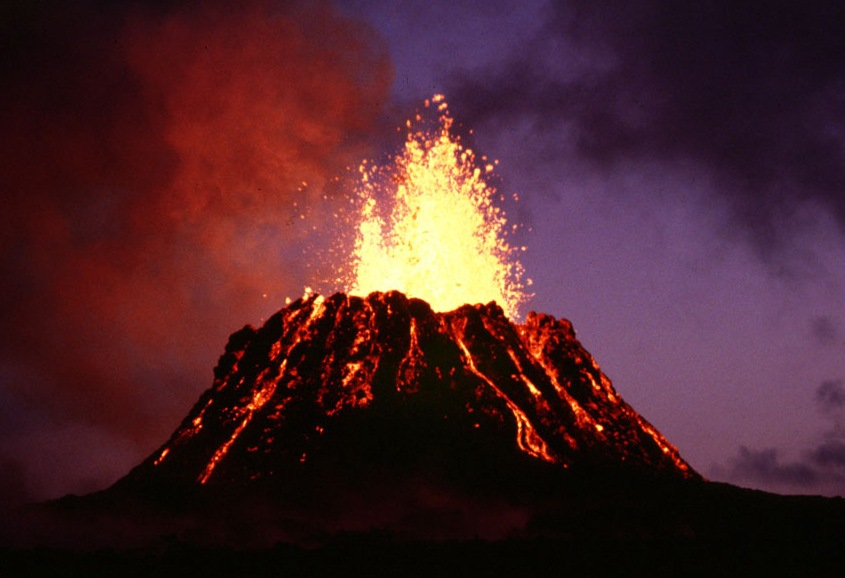
\includegraphics[width=0.55\linewidth]{images/book3/b1-puu-oo-1983.jpg}
\par\smallskip{\small Uma fonte de lava no cone Pu\textquoteleft
u~\textquoteleft O\textquoteleft o, na zona de rifte leste do Kilauea, 29 de junho de 1983, no primeiro ano de uma erupção que durou décadas: lava basáltica, quente e fluida, lançada em jato e caindo de volta em torno da abertura. Foto: G.~E.~Ulrich, U.S. Geological Survey, domínio público
(Wikimedia Commons).}
\label{fig:b1:hotspots:puu-oo}
\end{omfigure}
% ledger: commons:puu-oo, pp1801:kilauea-rate

\begin{history}[Um referencial fixo para as placas]
Em 1963, John Tuzo Wilson explicou as ilhas havaianas, cada vez mais antigas ao longo de uma linha, por uma fonte de lava mantida no núcleo lento de uma célula de convecção do \omterm{def:b1:layered-earth:layers}{manto}, enquanto a parte superior, mais rápida, da célula levava o fundo do mar sobre ela. Em 1971 e 1972, W. Jason Morgan fez dessa fonte uma pluma, de cerca de \qty{150}{km} de largura, subindo da parte mais baixa do \omterm{def:b1:layered-earth:layers}{manto} e, portanto, quase fixa enquanto as placas se movem sobre ela; experimentos em tanques logo mostraram como tal pluma se parece. Os \omterm{def:b1:hotspots:hotspot}{pontos quentes} tornaram-se um referencial no qual as placas podiam ser medidas contra o \omterm{def:b1:layered-earth:layers}{manto}, e não apenas umas contra as outras. Meio século depois, sabe-se que o referencial deriva, o \omterm{def:b1:hotspots:hotspot}{ponto quente} do Havaí entre outros, mas devagar o bastante para que as trilhas do Pacífico ainda deem o movimento da placa sobre o \omterm{def:b1:layered-earth:layers}{manto} com precisão de poucos graus e de poucos centímetros por ano, como mostrou o ajuste deste capítulo.
\end{history}
% ledger: hist:plumes, tarduno:emperor

\section{Grandes províncias ígneas}\label{sec:b1:hotspots:lips}

\begin{definition}[Grande província ígnea]\label{def:b1:hotspots:lip}
Uma \emph{grande província ígnea}\index{grande província ígnea} (LIP) é um acúmulo de rocha ígnea, sobretudo basalto, que não se forma por espalhamento comum em uma dorsal, cobre mais de \qty{e5}{km^2}, contém mais de \qty{e5}{km^3} e foi colocada em no máximo cerca de 50 milhões de anos, a maior parte em pulsos de 1 a 5 milhões de anos que carregam mais de três quartos de seu volume. Em terra, as LIPs são em geral basaltos de inundação; nos oceanos, platôs oceânicos.
\end{definition}

Uma LIP típica cobre cerca de um milhão de quilômetros quadrados e contém cerca de um milhão de quilômetros cúbicos de lava, a maior parte erupcionada em cerca de um milhão de anos ou menos. Suas lavas estão empilhadas em fluxos quase planos, que a erosão corta em degraus, as \emph{armadilhas} de seus nomes. A tabela lista as principais das últimas 260 milhões de anos.
% ledger: be08:definition, cr03:summary

\begin{omfigure}
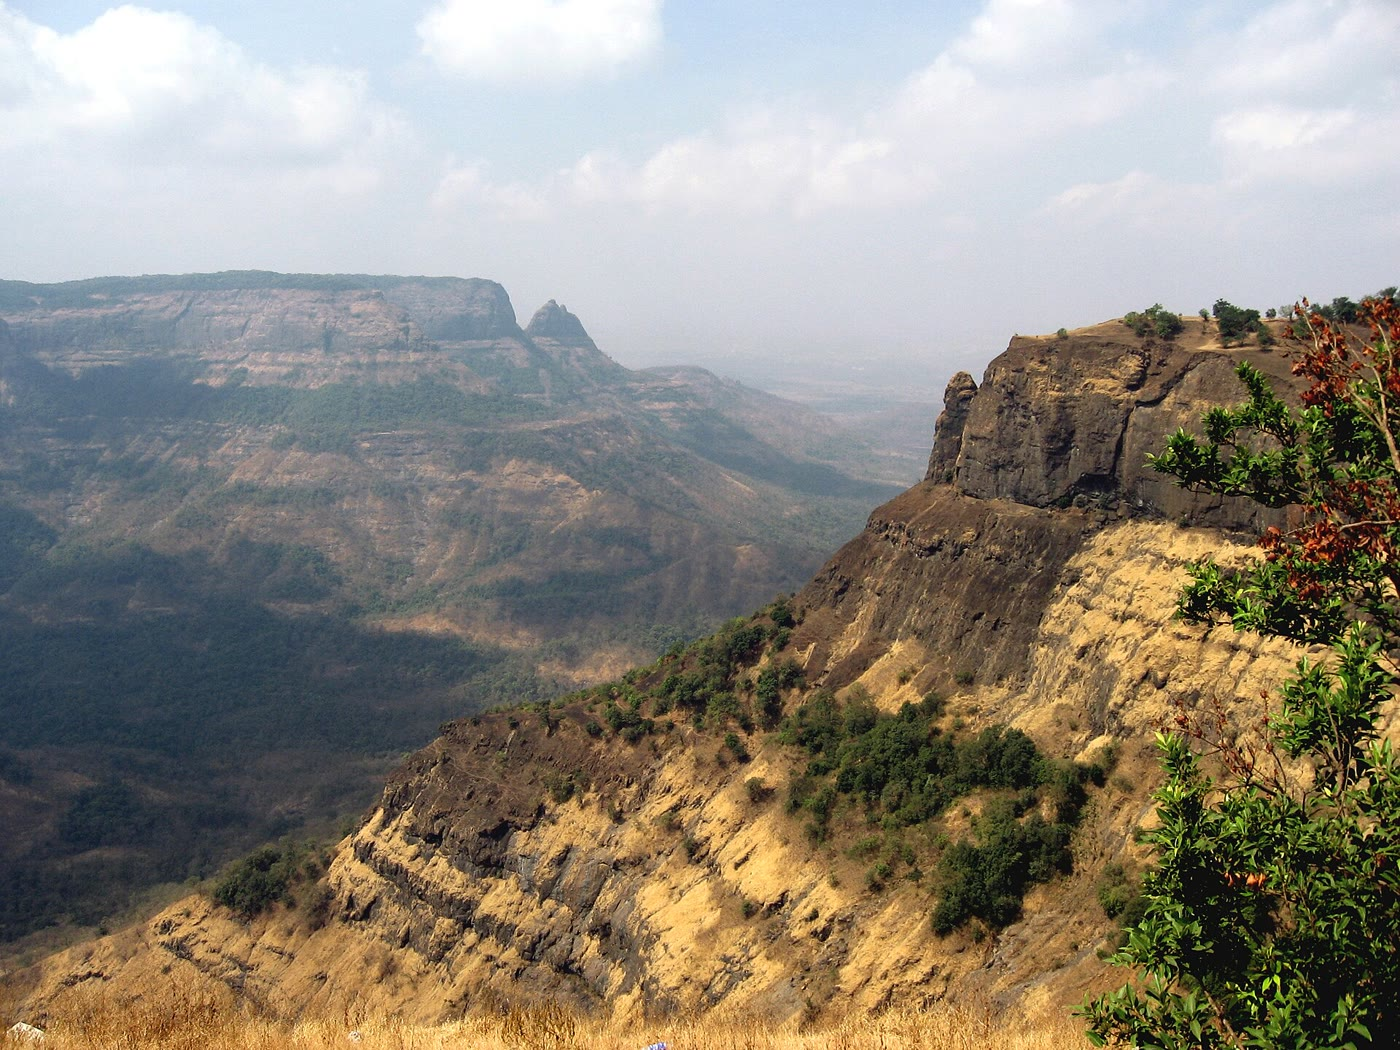
\includegraphics[width=0.55\linewidth]{images/book3/b1-deccan-matheran.jpg}
\par\smallskip{\small Os Ghats Ocidentais perto de Matheran, Índia: colinas de topo plano cortadas em uma pilha de fluxos de lava quase horizontais das Armadilhas do Decão, cujas camadas resistentes formam os degraus das encostas. Foto: Nicholas
(Nichalp), CC BY-SA 2.5 (Wikimedia Commons).}
\label{fig:b1:hotspots:deccan}
\end{omfigure}
% ledger: commons:matheran

\begin{center}
\small
\begin{tabular}{llll}
\hline
província & idade (Ma) & área (\unit{Mkm^2}) & volume inicial (\unit{Mkm^3})\\
\hline
Columbia River & 16 & 0.2 & 0.2\\
Etiópia--Iêmen & 30 & 0.7 & 1.2\\
Atlântico Norte & 61 e 56 & 1.2 & mais de 2\\
Decão & 65.5 & 0.5 (outrora 1.8) & 2 a 4\\
Ontong Java & 122 e 90 & 2 & 44 (\omterm{def:b1:layered-earth:layers}{crosta} inteira)\\
Paraná--Etendeka & 133 & 1.5 (outrora mais de 2) & mais de 2.3\\
Karoo--Ferrar & 183 & 3.1 & mais de 2.5\\
Atlântico Central (CAMP) & 201 & outrora até 7 & mais de 2\\
Armadilhas Siberianas & 250 & 0.4 (outrora mais de 4) & mais de 3\\
Emeishan & 259 & 0.5 (outrora 2 a 5) & mais de 1\\
\hline
\end{tabular}
\par\smallskip{\small Idades médias; áreas como são hoje, e como foram primeiro erupcionadas onde existe uma estimativa; volumes de lava como foram primeiro erupcionados, exceto para o Platô Ontong Java, cuja cifra conta toda a sua \omterm{def:b1:layered-earth:layers}{crosta} espessada. Dados: V.~Courtillot e P.~Renne (2003).}
\end{center}
% ledger: cr03:table

\noindent O modelo de pluma esboçado em \cref{sec:b1:hotspots:plumes} explica tanto o tamanho quanto a pressa: uma cabeça de pluma de centenas de quilômetros de largura alcança a base da \omterm{def:b1:layered-earth:lithosphere}{litosfera}, descomprime e funde, e inunda a superfície; em seguida a cauda continua a construir uma \omterm{def:b1:hotspots:track}{trilha de ponto quente} comum. Várias províncias são consideradas o extremo antigo de uma trilha ainda viva: as Armadilhas do Decão e o \omterm{def:b1:hotspots:hotspot}{ponto quente} da Reunião, o Paraná--Etendeka e Tristão da Cunha, ligados pela Cordilheira de Walvis, e os basaltos do Rio Columbia e Yellowstone.
% ledger: cr03:deccan (Reunion hot spot, plume-head model), be08:ojmh (Parana-Etendeka-Walvis-Tristan), pm90:track (Columbia River basalts)

As Armadilhas do Decão, no centro-oeste da Índia, são uma pilha de fluxos de lava com cerca de \qty{2500}{m} de espessura, dos quais pelo menos \qty{1800}{m} foram erupcionados perto de 65.5 milhões de anos atrás, em muito menos de um milhão de anos; hoje cobrem cerca de \qty{0.5}{\mega km^2}, talvez \qty{1.8}{\mega km^2} antes da erosão. O Platô Ontong Java, no sudoeste do Pacífico, é o maior de todos os platôs oceânicos: cobre cerca de \qty{2}{\mega km^2}, e sua \omterm{def:b1:layered-earth:layers}{crosta}, com cerca de \qty{36}{km} de espessura, contém cerca de \qty{44}{\mega km^3} de rocha ígnea. Os platôs de Manihiki e Hikurangi, hoje distantes dele pelo fundo do mar mais jovem, podem ter se formado com ele como um único platô. A Província Magmática do Atlântico Central, erupcionada cerca de 201 milhões de anos atrás, quando o Atlântico começou a abrir-se, está hoje espalhada, como lavas, diques e soleiras, por quatro continentes: o leste da América do Norte, o nordeste da América do Sul, a África Ocidental e o sudoeste da Europa; pode ter coberto até \qty{7}{\mega km^2}.
% ledger: cr03:deccan, cr03:table, cr03:ontong-java, be08:ojmh, cr03:camp


Várias províncias coincidem no tempo com as grandes extinções em massa que a biologia descreve: as Armadilhas Siberianas com a maior de todas, no fim do Permiano; a província do Atlântico Central com o fim do Triássico; as Karoo--Ferrar com uma extinção no Jurássico Inferior; a Emeishan com uma no Permiano Médio; e as Armadilhas do Decão com o fim do Cretáceo. As quatro maiores extinções dos últimos 260 milhões de anos caem, tão de perto quanto as datas permitem dizer, em uma dessas províncias, e uma ligação causal é tida como a mais provável. Os mecanismos propostos são atmosféricos: aerossóis de sulfato que resfriam o clima por um curto tempo, dióxido de carbono que o aquece por muito mais tempo, e oceanos privados de oxigênio. No caso do fim do Cretáceo, as erupções do Decão começaram antes do impacto de Chicxulub e continuaram depois dele; uma revisão dos registros do limite concluiu em 2010 que o impacto desencadeou a extinção.
% ledger: cr03:table, cr03:summary, cr03:deccan, schulte:kpg

Nem todo vulcanismo longe dos limites das placas precisa de pluma. Pequenos campos vulcânicos crescem onde uma placa é distendida ou fraturada, e as cadeias sem uma \omterm{def:b1:hotspots:track}{progressão de idade} clara podem ser alimentadas pelo \omterm{def:b1:layered-earth:layers}{manto} superior; esse é o modelo da hipótese das placas em ação. O que as ilhas oceânicas se tornam depois que o \omterm{def:b1:hotspots:hotspot}{ponto quente} as deixou, à medida que afundam, se desgastam e formam recifes, pertence ao Livro 4.
% ledger: fn03:plate-hypothesis

\section{Exercícios}

\begin{exercise}[$\star$]\label{exo:b1:hotspots:1}
(a) O Mauna Kea se ergue \qty{4205}{m} acima do nível do mar, e o fundo do mar longe da cadeia havaiana fica a \qty{5274}{m} de profundidade. Calcule quanto o vulcão se eleva acima desse fundo. Explique por que sua altura real, medida a partir da base, é ainda maior. (b) O Mauna Loa contém cerca de \qty{74000}{km^3}. Quanto tempo levaria para construí-lo com o suprimento atual do Kilauea, \qty{0.1}{km^3} por ano, e com a taxa média de toda a cadeia, \qty{0.025}{km^3} por ano? (c) A erupção do Pu\textquoteleft
u~\textquoteleft O\textquoteleft o lançou cerca de \qty{0.12}{km^3} por ano de 1983 a 2002. Qual é esse volume, e que fração do Mauna Loa ele representa?
% ledger: pp1801:volumes, pp1801:kilauea-supply, pp1801:chain-volume, pp1801:kilauea-rate; 5274 m from hotspots.py
\end{exercise}

\begin{exercise}[$\star$]\label{exo:b1:hotspots:2}
Uma placa gira sobre os \omterm{def:b1:hotspots:hotspot}{pontos quentes} a \qty{0.92}{\degree\per\Myr}. Tome $R = \qty{6371}{km}$. (a) Exprima $\omega$ em radianos por milhão de anos. (b) Calcule a velocidade, em \unit{mm.yr^{-1}}, dos \omterm{def:b1:hotspots:hotspot}{pontos quentes} a \ang{30}, \ang{60}, \ang{90} e \ang{108.0} do polo. (c) Por que a velocidade do Havaí, a \ang{108.0}, é menor que a de \ang{90}?
\end{exercise}

\begin{exercise}[$\star$]\label{exo:b1:hotspots:3}
(a) Calcule a espessura média das Armadilhas do Decão como são hoje, \qty{1}{\mega km^3} sobre \qty{0.5}{\mega km^2}, e da província do Atlântico Central, \qty{2}{\mega km^3} sobre \qty{7}{\mega km^2}. (b) Compare com a espessura da seção do Decão, \qty{2500}{m}. (c) Por que a espessura média da província do Atlântico Central diz pouco sobre a espessura de suas pilhas de lava?
% ledger: cr03:table, cr03:deccan, cr03:camp
\end{exercise}

\begin{exercise}[$\star$]\label{exo:b1:hotspots:4}
Uma rocha de pluma \qty{250}{K} mais quente que o \omterm{def:b1:layered-earth:layers}{manto} ao redor tem
$\alpha = \qty{3.2e-5}{K^{-1}}$ e $\rho_m = \qty{3300}{kg.m^{-3}}$. (a) Em quanto ela é mais leve, em \unit{kg.m^{-3}}? (b) Que espessura dessa rocha, espalhada sob a placa, sustentaria isostaticamente uma elevação de \qty{690}{m} de altura sob o mar ($\rho_w = \qty{1000}{kg.m^{-3}}$)?
% ledger: herzberg:tp (200-300 K), parsons:plate-model (alpha)
\end{exercise}

\begin{exercise}[$\star\star$]\label{exo:b1:hotspots:5}
Dois \omterm{def:b1:hotspots:hotspot}{pontos quentes} estão sobre o equador, A em \ang{0}\,L e B em \ang{90}\,L, e ambas as trilhas seguem exatamente para o oeste (\omterm{def:b1:spherical-astronomy:horizontal}{azimute} \ang{270}). (a) Calcule os vetores das trilhas $\vec t_A$ e $\vec t_B$. (b) Calcule $\vec t_A\times\vec t_B$. (c) Aplique a regra de sinal de \cref{prop:b1:hotspots:two-tracks}: onde está o \omterm{def:b1:plate-kinematics:euler-pole}{polo de Euler}? Explique o resultado sem cálculo. (d) Se A se move a \qty{50}{mm.yr^{-1}}, qual é $\omega$ em graus por milhão de anos?
\end{exercise}

\begin{exercise}[$\star\star$]\label{exo:b1:hotspots:6}
Três \omterm{def:b1:hotspots:hotspot}{pontos quentes} de uma mesma placa estão às distâncias $x = R\sin\Delta = 3000$, 5000
e \qty{6000}{km} do eixo de rotação, e se movem a 30, 48 e
\qty{57}{mm.yr^{-1}}. (a) Ajuste $v = \omega x$ pelos mínimos quadrados e dê $\omega$ em radianos e em graus por milhão de anos. (b) Calcule os resíduos. (c) Por que a reta deve passar pela origem?
\end{exercise}

\begin{exercise}[$\star\star$]\label{exo:b1:hotspots:7}
Uma elevação de seção transversal \qty{3e8}{m^2} envolve uma \omterm{def:b1:hotspots:track}{trilha de ponto quente} sobre uma placa que se move a \qty{50}{mm.yr^{-1}}. Tome $\rho_m - \rho_w = \qty{2300}{kg.m^{-3}}$,
$c_p = \qty{910}{J.kg^{-1}.K^{-1}}$ e $\alpha = \qty{3.2e-5}{K^{-1}}$. (a) Calcule seu fluxo de flutuabilidade e seu \omterm{def:b1:heat-budget:heat-flow}{fluxo de calor}. (b) Compare com o do Havaí, \qty{3240}{kg.s^{-1}}. (c) Dois \omterm{def:b1:hotspots:hotspot}{pontos quentes} têm a mesma elevação; um deles está sob uma placa que se move duas vezes mais depressa. Qual pluma é mais forte?
\end{exercise}

\begin{exercise}[$\star\star$]\label{exo:b1:hotspots:8}
Ao longo da trilha de Yellowstone, as erupções de caldeira começaram no campo vulcânico McDermitt há 16.1 milhões de anos e no campo de Picabo, a cerca de \qty{350}{km} para nordeste, há 10.3 milhões de anos; desde então elas se deslocam à velocidade de $\qty[uncertainty-mode=separate]{2.9 \pm 0.5}{cm}$ por ano, em direção a
N\,\ang{54}\,L. (a) Com que velocidade média o vulcanismo migrou de McDermitt para Picabo? (b) Compare as duas velocidades com a da placa sobre o \omterm{def:b1:hotspots:hotspot}{ponto quente}, \qty[uncertainty-mode=separate]{26 \pm 5}{mm.yr^{-1}} em direção a \ang{235}. (c) O rumo da trilha jovem é o esperado? (d) A parte mais antiga da trilha situa-se em uma região que foi distendida à medida que o vulcanismo passava. Como isso pode explicar a diferença?
% ledger: pm90:track, data:b3-hotspots
\end{exercise}

\begin{exercise}[$\star\star$]\label{exo:b1:hotspots:9}
A pluma havaiana carrega cerca de \qty{9.2e10}{W} de calor em excesso. (a) Se tudo isso saísse pelos \qty{1000}{km} por \qty{1000}{km} de fundo do mar mais próximos do \omterm{def:b1:hotspots:hotspot}{ponto quente}, de quanto subiria ali o \omterm{def:b1:heat-budget:heat-flow}{fluxo de calor}? (b) Compare com o excesso observado, de no máximo 5 a \qty{10}{mW.m^{-2}}. (c) Quanto tempo leva o calor para se difundir por uma placa de \qty{100}{km} de espessura ($\kappa = \qty{e-6}{m^2.s^{-1}}$)? Quanto tempo a placa leva para atravessar \qty{1000}{km} a \qty{92}{mm.yr^{-1}}? Conclua.
% ledger: vh89:swell-heat
\end{exercise}

\begin{exercise}[$\star\star\star$]\label{exo:b1:hotspots:10}
As Armadilhas do Decão contêm cerca de \qty{e6}{km^3} de lava. Suponha que ela veio de uma cabeça de pluma esférica, da qual um décimo fundiu. (a) Qual eram o volume e o raio da cabeça? (b) Achatada sob a \omterm{def:b1:layered-earth:lithosphere}{litosfera} em um disco de \qty{100}{km} de espessura, que diâmetro teria a cabeça? Compare sua área com a área que as Armadilhas podem ter coberto, \qty{1.8}{\mega km^2}. (c) Se a lava foi erupcionada em um milhão de anos, compare sua taxa com o suprimento atual do Kilauea, \qty{0.1}{km^3} por ano. (d) Por que uma cabeça de pluma deve ser grande, enquanto a cauda que a segue é estreita?
% ledger: cr03:table, pp1801:kilauea-supply
\end{exercise}

\begin{exercise}[$\star\star\star$]\label{exo:b1:hotspots:11}
Entre 81 e 47 milhões de anos atrás, o \omterm{def:b1:hotspots:hotspot}{ponto quente} havaiano se deslocou para o sul a mais de \qty{40}{mm.yr^{-1}}. (a) Tomando \qty{40}{mm.yr^{-1}}, quanto ele se deslocou?
(b) Suponha que, nesse meio-tempo, a placa se movesse a \qty{80}{mm.yr^{-1}} em direção a \ang{340} sobre o \omterm{def:b1:layered-earth:layers}{manto} profundo. Com $x$ para leste e $y$ para norte, calcule a velocidade da placa em relação ao \omterm{def:b1:hotspots:hotspot}{ponto quente}, que se deslocava, sua velocidade e seu \omterm{def:b1:spherical-astronomy:horizontal}{azimute}. (c) Em que porcentagem, e em quantos graus, uma trilha construída então representaria mal o movimento da placa sobre o \omterm{def:b1:layered-earth:layers}{manto} profundo?
% ledger: tarduno:emperor
\end{exercise}

\begin{exercise}[$\star\star\star$]\label{exo:b1:hotspots:12}
(a) Um basalto de inundação de \qty{e6}{km^3} esfria de cerca de \qty{1300}{\celsius} até a temperatura da superfície. Com uma capacidade térmica volumétrica de \qty{3}{MJ.m^{-3}.K^{-1}}, quanto calor ele libera (despreze o calor latente de cristalização)? (b) Distribuída ao longo de um milhão de anos, que potência é essa? Compare com a da pluma havaiana, \qty{9.2e10}{W}, e com os \qty{47}{TW} de toda a Terra. (c) Uma cabeça de pluma também aquece a base da \omterm{def:b1:layered-earth:lithosphere}{litosfera} sem fundir toda ela. A potência do item (b) é um limite superior ou inferior do calor trazido pela cabeça?
% ledger: delaney86:properties (Book 2 row, 2-3 MJ/m3/K), dd10:total; 1300 degC is an exercise value
\end{exercise}

\section{Problema: o velocímetro da placa do Pacífico}

\begin{problem}[{Problema de fim de semana --- o polo de Euler da placa do Pacífico a partir de duas
trilhas de pontos quentes, sua taxa a partir de uma terceira medida, um teste com outros pontos quentes
e a flutuabilidade e o suprimento da pluma havaiana}]
\label{pb:b1:hotspots:1}
% values: calc/ch15.py; ledger: data:b3-hotspots, data:etopo1, pp1801:kilauea-supply, pp1801:volumes,
% pp1801:chain-volume, delaney86:properties, parsons:plate-model, dd10:total, data:pb2002 (ridge_budget.py), cd87:rate
Morgan e Morgan dão o \omterm{def:b1:hotspots:hotspot}{ponto quente} do Havaí em \ang{19.0}\,N, \ang{155.2}\,O, com uma trilha em direção a $\ang{304}\pm\ang{3}$ e uma velocidade de \qty[uncertainty-mode=separate]{92 \pm 3}{mm.yr^{-1}}, e o \omterm{def:b1:hotspots:hotspot}{ponto quente} de Louisville em \ang{53.6}\,S, \ang{140.6}\,O, com uma trilha em direção a $\ang{316}\pm\ang{5}$ e uma velocidade de \qty[uncertainty-mode=separate]{67 \pm 5}{mm.yr^{-1}}. Use os eixos e os vetores $\vec e$, $\vec n$, $\vec t$ da \cref{sec:b1:hotspots:tracks}, com $R = \qty{6371}{km}$. Dê as componentes com quatro casas decimais.

\medskip
\noindent\textbf{Parte I --- O polo a partir de duas trilhas.}
\begin{enumerate}
  \item Calcule $\vec r$, $\vec e$ e $\vec n$ no Havaí, depois o vetor da trilha
        $\vec t_H$.
  \item Faça o mesmo em Louisville: $\vec r_L$, $\vec e$, $\vec n$ e
        $\vec t_L$.
  \item Verifique que $\vec t_H$ é um vetor unitário perpendicular a $\vec r_H$.
  \item Calcule $\vec t_H\times\vec t_L$ e seu comprimento. Que ângulo formam os dois vetores das trilhas?
  \item Normalize o produto vetorial e aplique a regra de sinal de
        \cref{prop:b1:hotspots:two-tracks}.
  \item Dê a \omterm{def:b1:spherical-astronomy:geographic}{latitude} e a \omterm{def:b1:spherical-astronomy:geographic}{longitude} do \omterm{def:b1:plate-kinematics:euler-pole}{polo de Euler} da placa do Pacífico em relação aos \omterm{def:b1:hotspots:hotspot}{pontos quentes}.
\end{enumerate}

\medskip
\noindent\textbf{Parte II --- A taxa.}
\begin{enumerate}[resume]
  \item Calcule as distâncias angulares $\Delta_H$ e $\Delta_L$ do polo aos dois \omterm{def:b1:hotspots:hotspot}{pontos quentes}.
  \item Calcule $(\vec p\times\vec r_L)\cdot\vec t_L$. Explique por que ele é igual a
        $\sin\Delta_L$, e o que seu sinal diz sobre o movimento em Louisville.
  \item A partir da velocidade em Louisville, calcule $\omega$ em radianos e em graus por milhão de anos.
  \item Quanto tempo a placa do Pacífico leva para dar uma volta completa em torno deste polo?
  \item O polo dos mínimos quadrados das quinze trilhas do Pacífico situa-se em
        \ang{63.78}\,S, \ang{112.48}\,L, com \qty{0.92}{\degree\per\Myr}. Calcule o ângulo entre os dois polos e compare as duas taxas.
\end{enumerate}

\medskip
\noindent\textbf{Parte III --- Um teste com três outros pontos quentes.} Morgan e Morgan dão o \omterm{def:b1:hotspots:hotspot}{ponto quente} da Sociedade (\ang{18.2}\,S, \ang{148.4}\,O)
\qty[uncertainty-mode=separate]{109 \pm 10}{mm.yr^{-1}}, Pitcairn
(\ang{25.4}\,S, \ang{129.3}\,O)
\qty[uncertainty-mode=separate]{90 \pm 15}{mm.yr^{-1}} e Cobb
(\ang{46.0}\,N, \ang{130.1}\,O)
\qty[uncertainty-mode=separate]{43 \pm 3}{mm.yr^{-1}}.
\begin{enumerate}[resume]
  \item Calcule a distância angular do polo da questão 6 a cada um dos três \omterm{def:b1:hotspots:hotspot}{pontos quentes}.
  \item Preveja as três velocidades com a taxa da questão 9.
  \item Quais previsões concordam com as velocidades medidas dentro de suas incertezas, e quais não concordam?
  \item Duas trilhas de rumos diferentes sempre dão um polo. Por que duas trilhas quase paralelas são uma escolha ruim?
\end{enumerate}

\medskip
\noindent\textbf{Parte IV --- A pluma e o velocímetro.} A elevação havaiana tem seção transversal de \qty{4.83e8}{m^2}. Tome
$\rho_m - \rho_w = \qty{2300}{kg.m^{-3}}$, $c_p = \qty{910}{J.kg^{-1}.K^{-1}}$
e $\alpha = \qty{3.2e-5}{K^{-1}}$.
\begin{enumerate}[resume]
  \item Converta \qty{92}{mm.yr^{-1}} para \unit{m.s^{-1}} e calcule o fluxo de flutuabilidade da pluma havaiana.
  \item Calcule o calor em excesso que ela carrega e compare com os \qty{47}{TW} que deixam a Terra.
  \item As dorsais produzem cerca de \qty{21}{km^3} de \omterm{def:b1:layered-earth:layers}{crosta} por ano ao longo de cerca de \qty{67000}{km}. Que comprimento de dorsal produz tanta \omterm{def:b1:layered-earth:layers}{crosta} quanto o suprimento do Kilauea, \qty{0.1}{km^3} por ano?
  \item Nesse ritmo, quanto tempo levaria para crescer o Mauna Loa, de cerca de \qty{74000}{km^3}?
  \item O \omterm{def:b1:hotspots:hotspot}{ponto quente} construiu cerca de \qty{2e6}{km^3} da cadeia em 81 milhões de anos. Calcule sua produção média e compare com o suprimento atual do Kilauea.
  \item Com o polo e a taxa das Partes I e II, calcule a velocidade que a trilha de Louisville prevê para a placa do Pacífico sobre o \omterm{def:b1:hotspots:hotspot}{ponto quente} havaiano.
  \item Compare com a velocidade medida, \qty[uncertainty-mode=separate]{92 \pm 3}{mm.yr^{-1}}: em quanto e em quantas incertezas-padrão elas diferem?
  \item A partir das idades dos vulcões havaianos, o Livro 2 encontrou \qty{9.1}{cm} por ano, e os autores das idades, ajustando a cadeia inteira, \qty{8.6}{cm} por ano. Compare essas médias, ao longo de dezenas de milhões de anos, com as duas velocidades dos \omterm{def:b1:hotspots:hotspot}{pontos quentes}.
  \item Com uma casa decimal, em centímetros por ano, que velocidade a trilha de Louisville dá à placa do Pacífico sobre o \omterm{def:b1:hotspots:hotspot}{ponto quente} havaiano?
\end{enumerate}
\end{problem}
